\chapter{METODOLOGIA}\label{CAP5}

O desenvolvimento do trabalho foi dividido em 3 etapas. A primeira etapa consistiu no desenvolvimento do software responsável por fazer a interação com a rede interna automotiva. A segunda etapa foi caracterizada pela configuração do \textit{Raspberry Pi} e instalação do software no dispositivo e a terceira etapa se refere à integração da aplicação com um serviço de computação em nuvem.

\section{DESENVOLVIMENTO DO SOFTWARE DE LEITURA}
O objetivo principal da concepção do software nesta fase inicial é possibilitar ao computador interagir com a rede interna veicular, enviando e recebendo dados através da interface \textit{OBD-II}. Para permitir a tradução de protocolos e tornar a comunicação simplificada, foi adquirido o dispositivo ELM327 com transmissão \textit{Bluetooth}, responsável por tratar das conversões dos protocolos automotivos presentes no conector \textit{OBD-II} para uma interface serial padrão, estabelecendo uma comunicação com o adaptador \textit{Bluetooth} do computador.

A construção do software foi feita utilizando-se a linguagem de programação Java na versão 8, juntamente com as seguintes tecnologias: \textit{BlueCove}, obd-java-api e JavaFx. \textit{BlueCove} é uma biblioteca Java que segue a especificação JSR-82, permitindo que uma aplicação acesse o adaptador \textit{Bluetooth} local para se comunicar com outros dispositivos \cite{bluecove}. obd-java-api, encontrada no repositório de Pires (https://github.com/pires/obd-java-api), é uma biblioteca que facilita a comunicação com o adaptador ELM327. O \textit{framework} JavaFx fornece um conjunto de pacotes que facilitam a criação de uma interface gráfica para uma aplicação \cite{pawlan}. A Figura \ref{Fig:tela_leitura_javafx} representa o protótipo do software desenvolvido utilizando o JavaFx.

\begin{figure}[!ht]
\centering
\caption{Imagem da tela de leitura prototipada.} 
{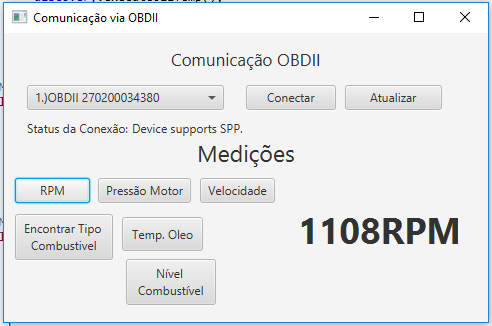
\includegraphics[scale=.75]{imagens/telaLeituraJavaFx.png}}\\
\makebox[\width]{Fonte: produzido pelo autor} \label{Fig:tela_leitura_javafx}
\end{figure}

\subsection{ARQUITETURA DO SOFTWARE}
O projeto foi desenvolvido utilizando-se o paradigma de programação orientada à objeto e o padrão \textit{Model-View-Controller (MVC)}, e devido a isso, foi necessário criar cinco pacotes para organizar as classes do código fonte. Os nomes dos pacotes criados foram: \textit{app}, \textit{bluetooth}, \textit{controller}, \textit{scanner}, e \textit{view}.

No pacote \textit{app} contém a classe \textit{AppStart} que é responsável por iniciar a aplicação e carregar a interface de usuário \textit{ScreenMonitor} contida no pacote \textit{view}. O pacote \textit{bluetooth} contém duas classes, uma chamada \textit{DiscoveryDevices} – responsável pela descoberta de dispositivos \textit{bluetooth} próximos – e outra chamada \textit{BluetoothConnection}, responsável por obter uma conexão \textit{bluetooth}. Dentro do pacote \textit{scanner} existem duas classes, uma com o nome \textit{ConnectToDevice}, que é responsável por estabelecer uma conexão com o dispositivo ELM327, e outra com o nome ELM327, representando o próprio dispositivo. O pacote \textit{view} contém o arquivo \textit{ScreenMonitor} no formato FXML, responsável por representar a interface de usuário. Por fim, o pacote \textit{controller} contém a classe \textit{ScreenMonitorController}, responsável por receber as entradas do usuário na interface e mapear as ações a serem tomadas pelo software. Na Figura \ref{Fig:diagrama_classe}, é possível observar a organização e estruturação das classes no projeto. A implementação do código das classes dos pacotes \textit{bluetooth} e \textit{scanner} poderá ser consultado em detalhes no capítulo \ref{anexoa} Anexo A.

\begin{figure}[!ht]
\centering
\caption{Diagrama de pacote exibindo a estrutura de pacotes do projeto com as respectivas classes.} 
{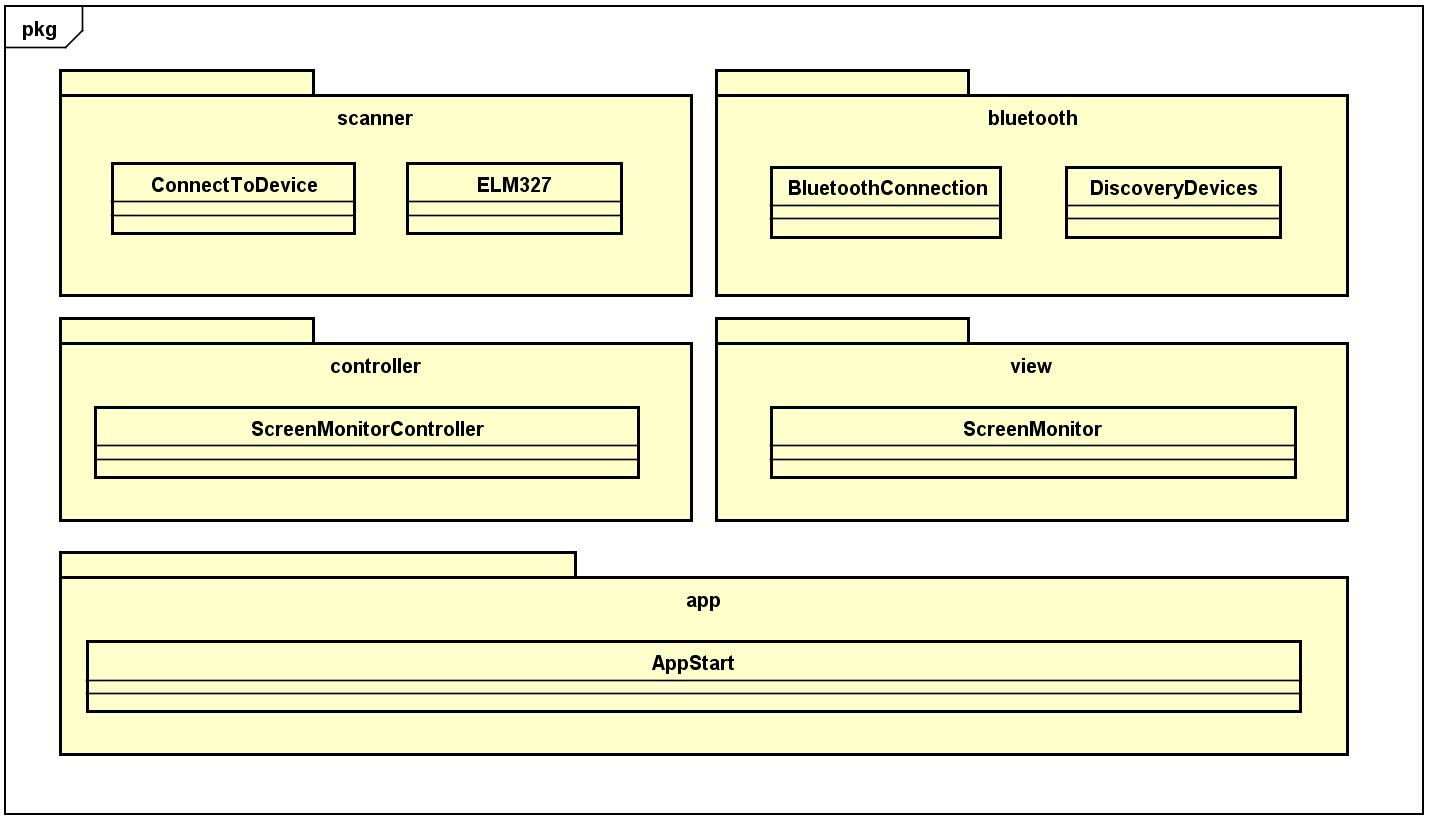
\includegraphics[scale=.42]{imagens/estruturacaoPacotes.png}}\\
\makebox[\width]{Fonte: produzido pelo autor} \label{Fig:diagrama_classe}
\end{figure}

No pacote \textit{scanner} existe a classe ELM327 (Figura \ref{Fig:elm327_class}) responsável por estabelecer a comunicação com o dispositivo de mesmo nome. Essa classe recebe como parâmetro em seu construtor dois objetos do tipo \textit{InputStream} e \textit{OutputStream}. Ela também contém alguns métodos, que são: \textit{disconnect} (Figura \ref{Fig:elm327_disconnect}), responsável por fechar a conexão dos objetos \textit{InputStream} e \textit{OutputStream}; \textit{readRpm} (Figura \ref{Fig:elm327_read_rpm}), responsável por efetuar a leitura da rotação por minuto (RPM) do motor, devolvendo uma \textit{string} no formato correto; \textit{readSpeed} (Figura \ref{Fig:elm327_read_speed}), responsável por efetuar a leitura da velocidade atual do automóvel, também retornando uma \textit{string} no formato Km/h; \textit{readFuelPressure} (Figura \ref{Fig:elm327_read_fuel_pressure}), responsável por obter a pressão do combustível em uma \textit{string}, no formato Psi ou Kilopascal (kPa); \textit{readOilTemp} (Figura \ref{Fig:elm327_read_oil_temp}), responsável por ler a temperatura do óleo do motor e devolver uma \textit{string} com o valor em graus \textit{Celsius} ($^{\circ}$C); \textit{readFindFuelType} (Figura \ref{Fig:elm327_read_find_fuel_type}), responsável por encontrar qual tipo de combustível está sendo utilizado no tanque; \textit{readFuelLevel} (Figura \ref{Fig:elm327_read_fuel_level}), responsável por obter a informação referente ao nível de combustível presente no tanque, e por último, o método \textit{clearBuffer} (Figura \ref{Fig:elm327_clear_buffer}), que implementa vários comandos que reiniciam a conexão \textit{OBD}, limpam o eco e o cabeçalho, possibilitando apagar o \textit{buffer} presente no dispositivo ELM327 para realizar novas leituras. Todos os métodos pertencentes à esta classe, exceto o \textit{disconnect}, fazem uso de classes e métodos que pertencem à biblioteca obd-java-api. Desta forma, as classes e métodos contidos nesta biblioteca abstraem a implementação de comandos ‘AT’ e \textit{‘OBD’}, tornando a sua utilização simplificada, bastando apenas chamar o recurso a ser utilizado sem se preocupar com a forma de implementação da funcionalidade.

\begin{figure}[!ht]
\centering
\caption{Foto da classe ELM327.} 
{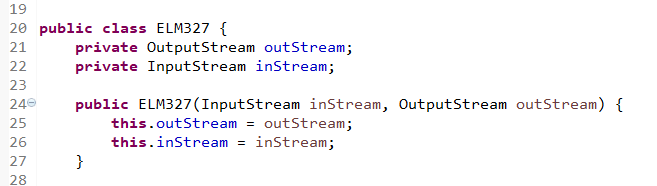
\includegraphics[scale=.70]{imagens/pacoteScanner-ELM327.png}}\\
\makebox[\width]{Fonte: produzido pelo autor} \label{Fig:elm327_class}
\end{figure}

\begin{figure}[!ht]
\centering
\caption{Foto do método \textit{disconnect} da classe ELM327.} 
{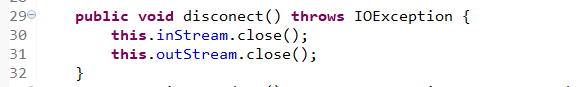
\includegraphics[scale=.70]{imagens/pacoteScanner-ELM327_disconnect.png}}\\
\makebox[\width]{Fonte: produzido pelo autor} \label{Fig:elm327_disconnect}
\end{figure}

\begin{figure}[!ht]
\centering
\caption{Foto do método \textit{readRpm} da classe ELM327.} 
{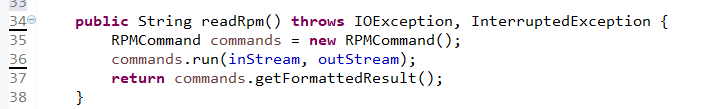
\includegraphics[scale=.85]{imagens/pacoteScanner-ELM327_readRpm.png}}\\
\makebox[\width]{Fonte: produzido pelo autor} \label{Fig:elm327_read_rpm}
\end{figure}

\begin{figure}[!ht]
\centering
\caption{Foto do método \textit{readSpeed} da classe ELM327.} 
{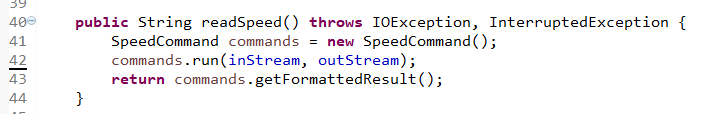
\includegraphics[scale=.85]{imagens/pacoteScanner-ELM327_readSpeed.png}}\\
\makebox[\width]{Fonte: produzido pelo autor} \label{Fig:elm327_read_speed}
\end{figure}

\begin{figure}[!ht]
\centering
\caption{Foto do método \textit{readFuelPressure} da classe ELM327.} 
{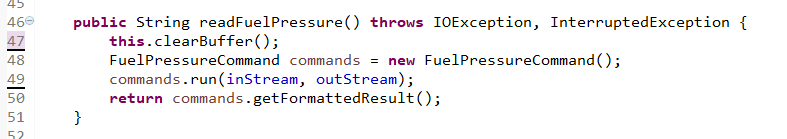
\includegraphics[scale=.80]{imagens/pacoteScanner-ELM327_readFuelPressure.png}}\\
\makebox[\width]{Fonte: produzido pelo autor} \label{Fig:elm327_read_fuel_pressure}
\end{figure}

\begin{figure}[!ht]
\centering
\caption{Foto do método \textit{readOilTemp} da classe ELM327.} 
{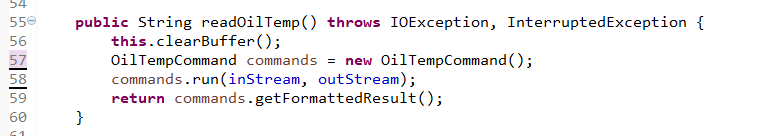
\includegraphics[scale=.85]{imagens/pacoteScanner-ELM327_readOilTemp.png}}\\
\makebox[\width]{Fonte: produzido pelo autor} \label{Fig:elm327_read_oil_temp}
\end{figure}

\begin{figure}[!ht]
\centering
\caption{Foto do método \textit{readFindFuelType} da classe ELM327.} 
{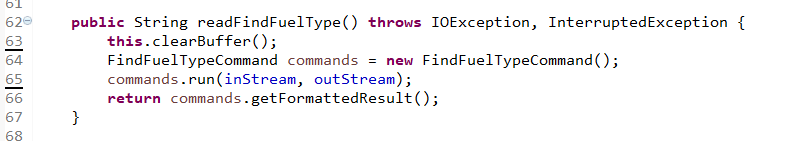
\includegraphics[scale=.80]{imagens/pacoteScanner-ELM327_readFindFuelType.png}}\\
\makebox[\width]{Fonte: produzido pelo autor} \label{Fig:elm327_read_find_fuel_type}
\end{figure}

\begin{figure}[!ht]
\centering
\caption{Foto do método \textit{readFuelLevel} da classe ELM327.} 
{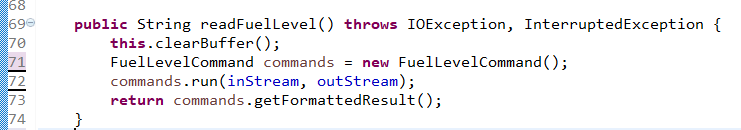
\includegraphics[scale=.70]{imagens/pacoteScanner-ELM327_readFuelLevel.png}}\\
\makebox[\width]{Fonte: produzido pelo autor} \label{Fig:elm327_read_fuel_level}
\end{figure}

\begin{figure}[!ht]
\centering
\caption{Foto do método \textit{clearBuffer} da classe ELM327.} 
{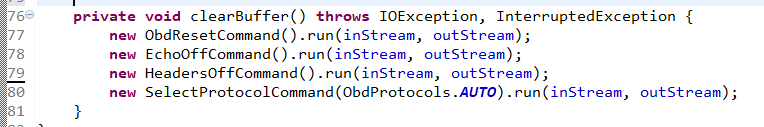
\includegraphics[scale=.70]{imagens/pacoteScanner-ELM327_clearBuffer.png}}\\
\makebox[\width]{Fonte: produzido pelo autor} \label{Fig:elm327_clear_buffer}
\end{figure}

Os pacotes \textit{view}, e \textit{controller} são implementações da arquitetura \textit{MVC}, que correspondem respectivamente à arquivos relacionados à interface de usuário, e à classes responsáveis por administrar as entradas dos usuários. Segundo \citeonline{medeirosmvc}, a arquitetura \textit{MVC} possui o controlador \textit{(Controller)} que gerencia as entradas dos usuários através das visões \textit{(Views)}, passando os comandos para os modelos \textit{(Models)} que gerencia diversos elementos de dados. Seguindo esta ideia, os pacotes que tem o papel de modelo, segundo esta arquitetura, seria o \textit{scanner} e o \textit{bluetooth} (Figura \ref{Fig:diagrama_mvc}).

\begin{figure}[!ht]
\centering
\caption{Representação da arquitetura \textit{MVC} do projeto.} 
{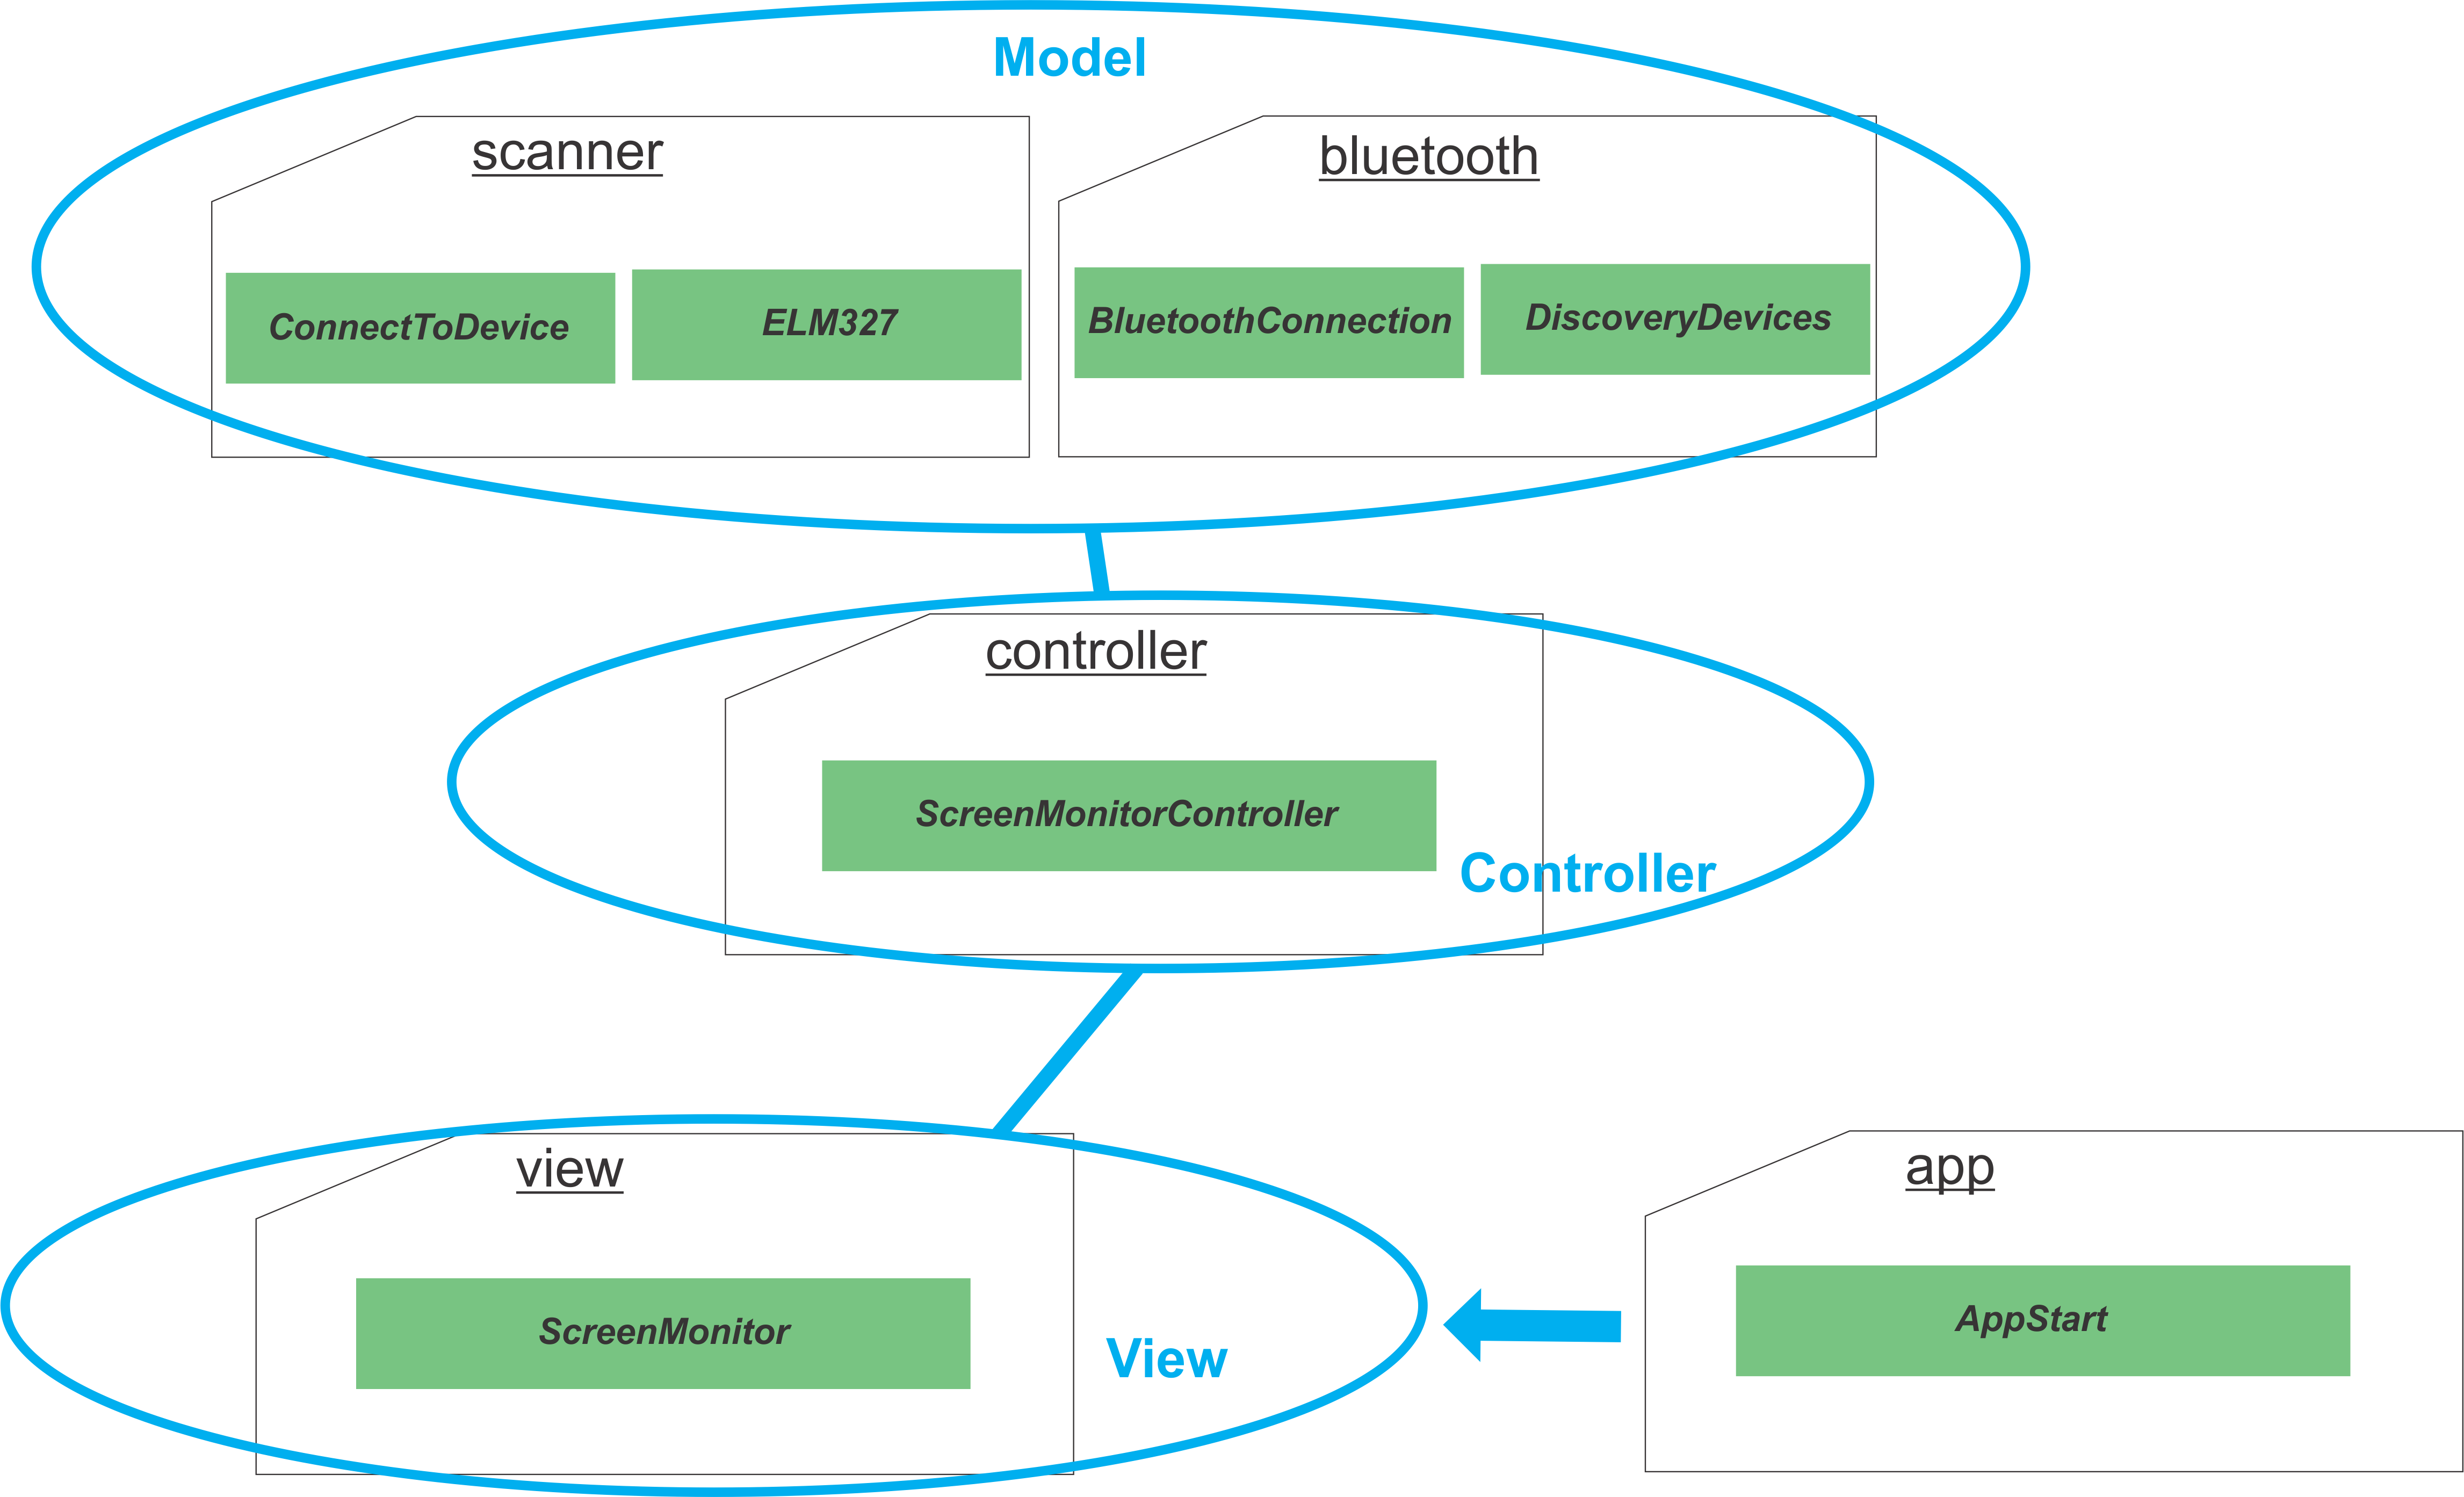
\includegraphics[scale=.40]{imagens/diagramaMvc.png}}\\
\makebox[\width]{Fonte: produzido pelo autor} \label{Fig:diagrama_mvc}
\end{figure}

\section{CONFIGURAÇÃO DO \textit{RASPBERRY PI} E INSTALAÇÃO DO SOFTWARE}
Primeiramente foi instalado a versão \textit{Jessie} do \textit{Raspbian}, com a atualização de 05 de julho de 2017 disponível em https://downloads.raspberrypi.org/raspbian/images/raspbian-2017-07-05/. O \textit{Raspbian}, conforme menciona \citeonline{long}, é uma distribuição do Linux baseada no Debian. Foi adquirido também, para o \textit{Raspberry} o display de 3.2 polegadas, modelo 3.2inch RPi Display com resolução de 320x240 pixels (Figura \ref{Fig:raspberry_display}). Este display é conectado na porta genérica de entrada e saída do \textit{Raspbery Pi} (porta GPIO - Figura \ref{Fig:raspberry_gpio}). O \textit{driver} de instalação do display está disponível em https://www.waveshare.com/wiki/3.2inch\_RPi\_LCD\_(B). De acordo com as instruções de instalação presentes neste site, os \textit{drivers} não são compatíveis com sistemas instalados pelo NOOBS. O sistema NOOBS, segundo o \citeauthor{raspberrypifoundation}, é um instalador de sistema operacional que contém o \textit{Raspbian}.

\begin{figure}[!ht]
\centering
\caption{Foto do display do \textit{Raspberry Pi}.} 
{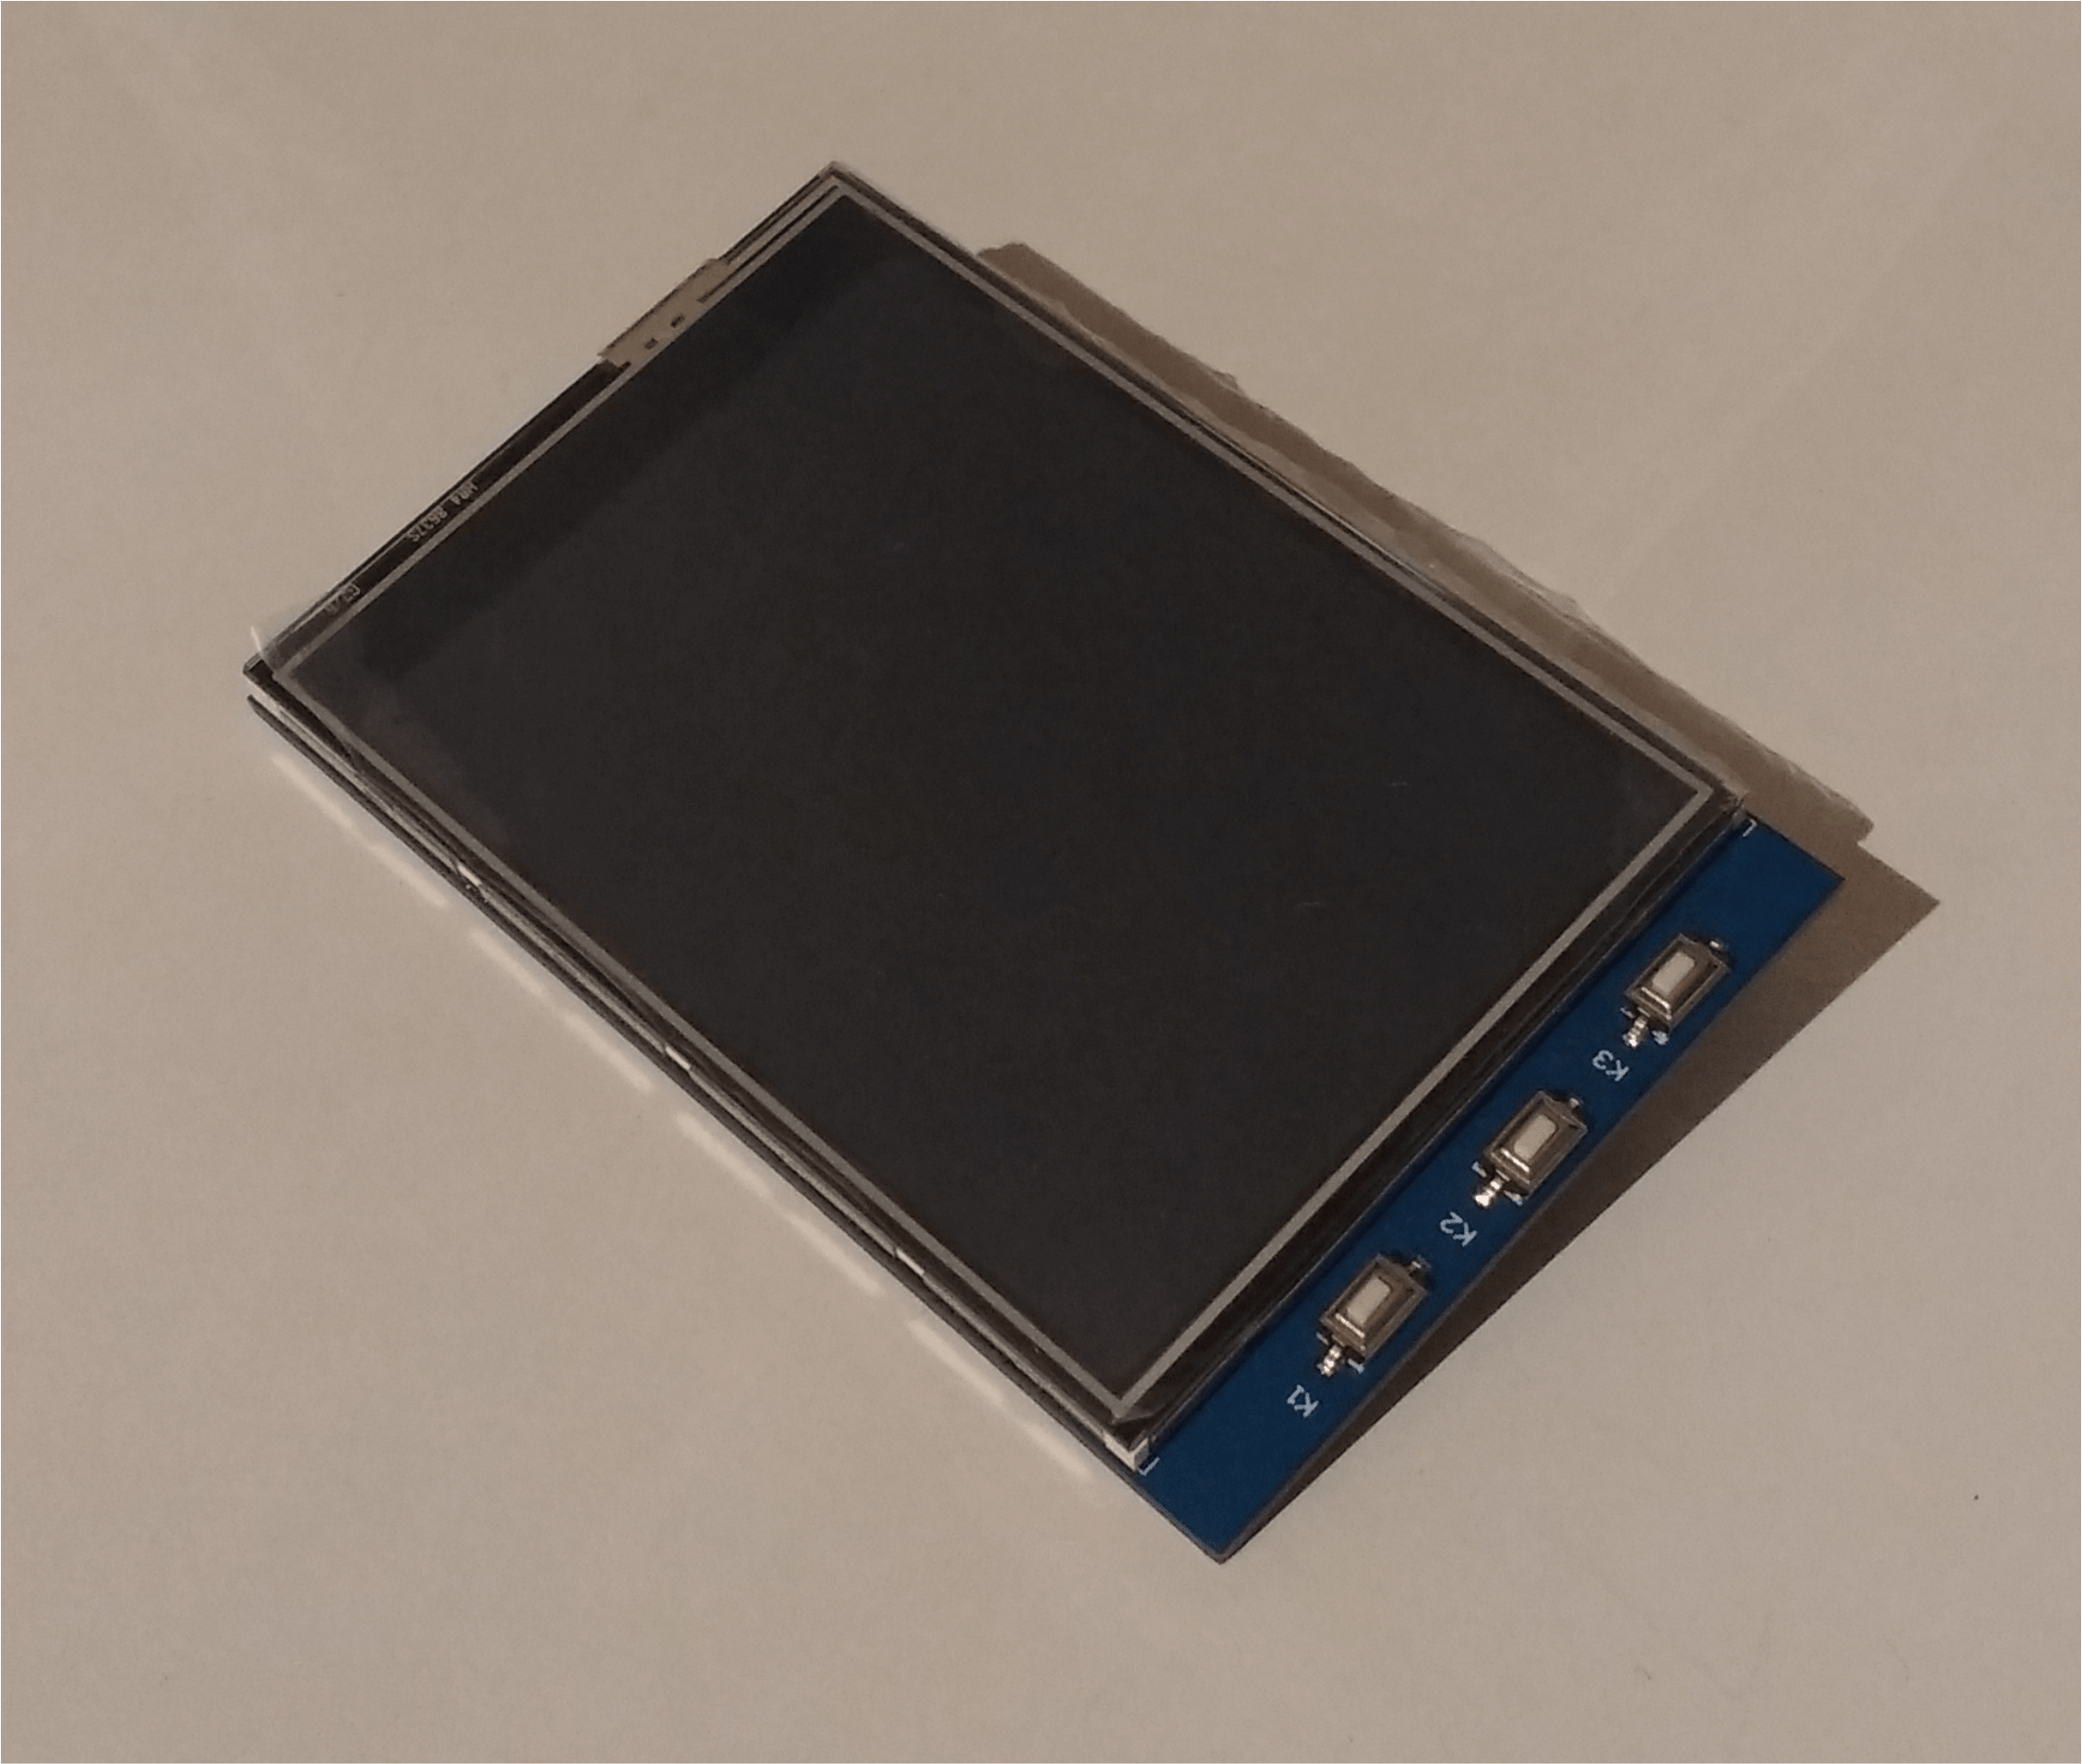
\includegraphics[scale=.12]{imagens/displayRaspberry-min.png}}\\
\makebox[\width]{Fonte: produzido pelo autor} \label{Fig:raspberry_display}
\end{figure}

\begin{figure}[!ht]
\centering
\caption{Porta GPIO do \textit{Raspberry Pi}.} 
{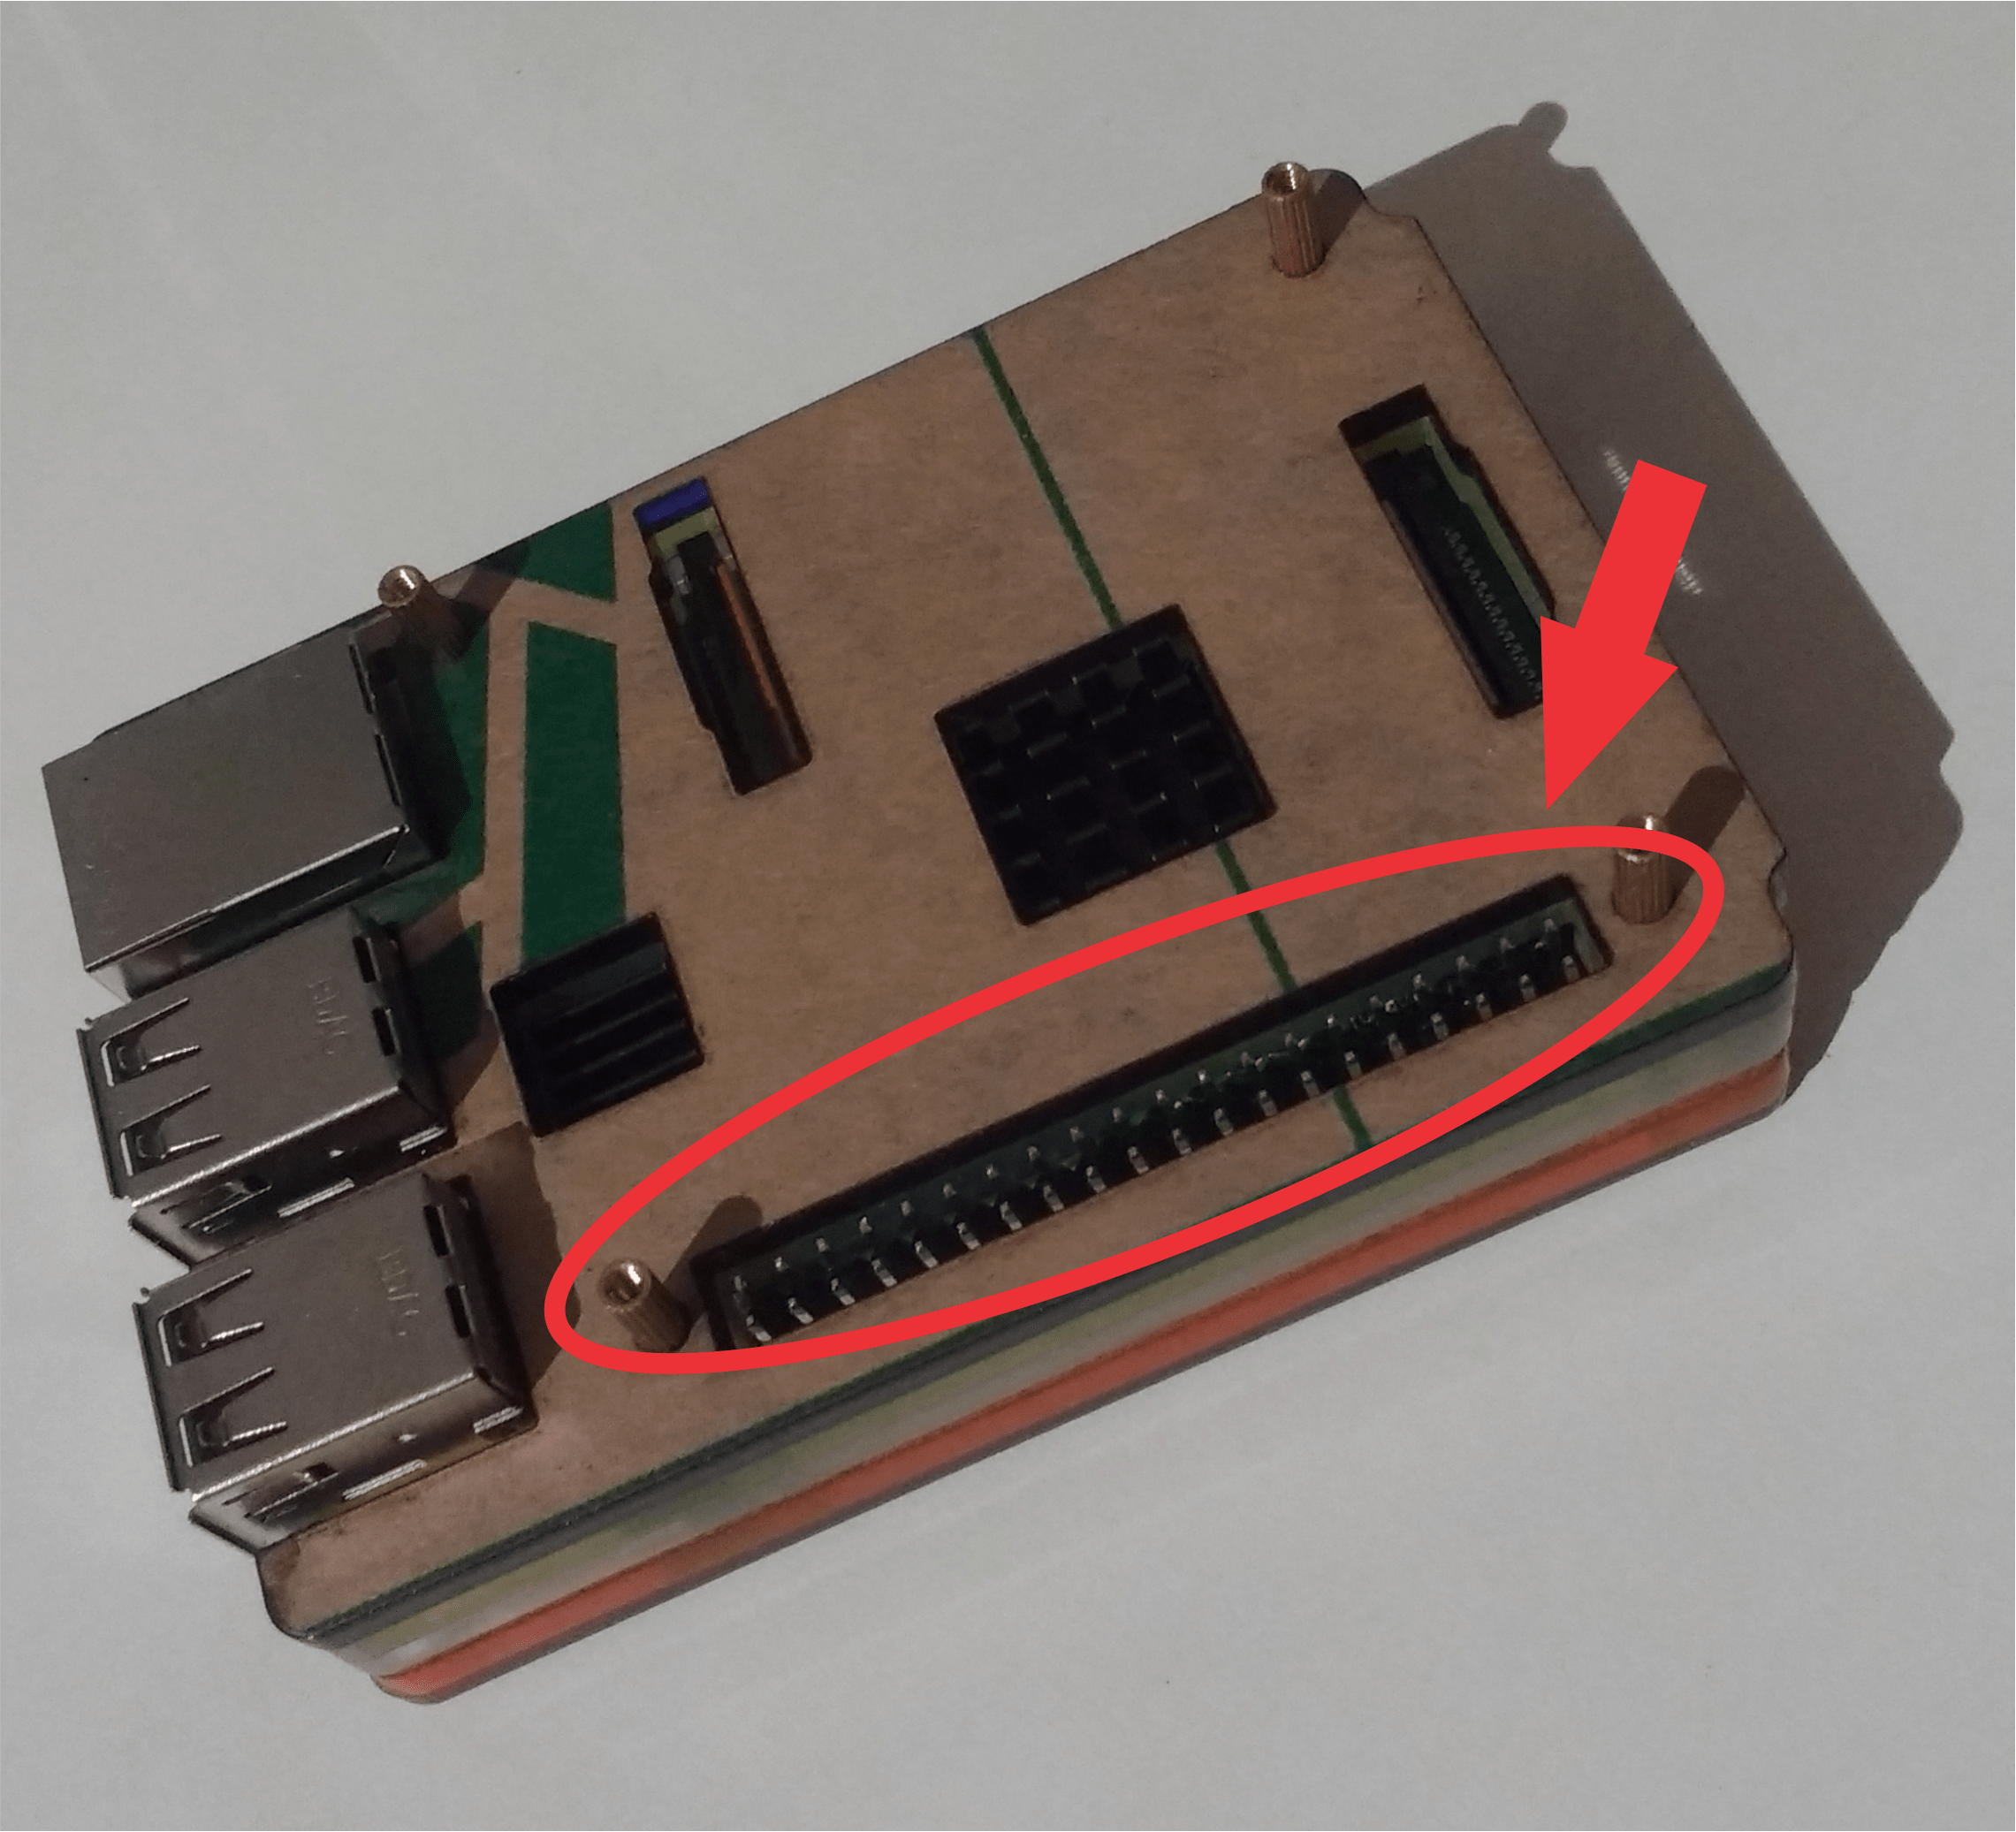
\includegraphics[scale=.12]{imagens/raspberryGPIO-min.png}}\\
\makebox[\width]{Fonte: produzido pelo autor} \label{Fig:raspberry_gpio}
\end{figure}

Para suportar a instalação e execução do software, depois de instalado e configurado o sistema operacional e o display, foi instalado o kit de desenvolvimento para Java na versão 8 (JDK 8) que incluía a máquina virtual (JRE) para rodar o projeto. Durante a fase de execução do projeto no ambiente do \textit{Raspberry}, notou-se que houve duas incompatibilidades. A primeira incompatibilidade identificada foi relacionada à biblioteca \textit{BlueCove}, pois ela não fornecia suporte para arquitetura ARM. A solução alternativa para contornar este problema foi encontrar uma versão da biblioteca construída para esta arquitetura. A segunda incompatibilidade foi relacionada ao \textit{framework} JavaFx, utilizado na interface gráfica. Foi identificado que nas configrações do \textit{Raspberry} não era possível executar o software utilizando esta tecnologia. Para solucionar este problema, foi necessário redesenhar a interface utilizando o \textit{Swing} – conjunto de componentes que permite a criação de interface gráfica –, que são inteiramente implementados na linguagem Java \cite{oracle}.

Foram feitas algumas modificações no projeto e na interface para se adequar à tela do \textit{Raspberry} de 3.2 polegadas. Como havia uma limitação de espaço de exibição no display, apenas as leituras de RPM, velocidade, tipo e pressão do combustível foram implementadas. A Figura \ref{Fig:raspberry_sistema} mostra o software adaptado à tela, sendo executado no \textit{Raspberry Pi}.

\begin{figure}[!ht]
\centering
\caption{Software sendo executado no \textit{Raspberry Pi}.} 
{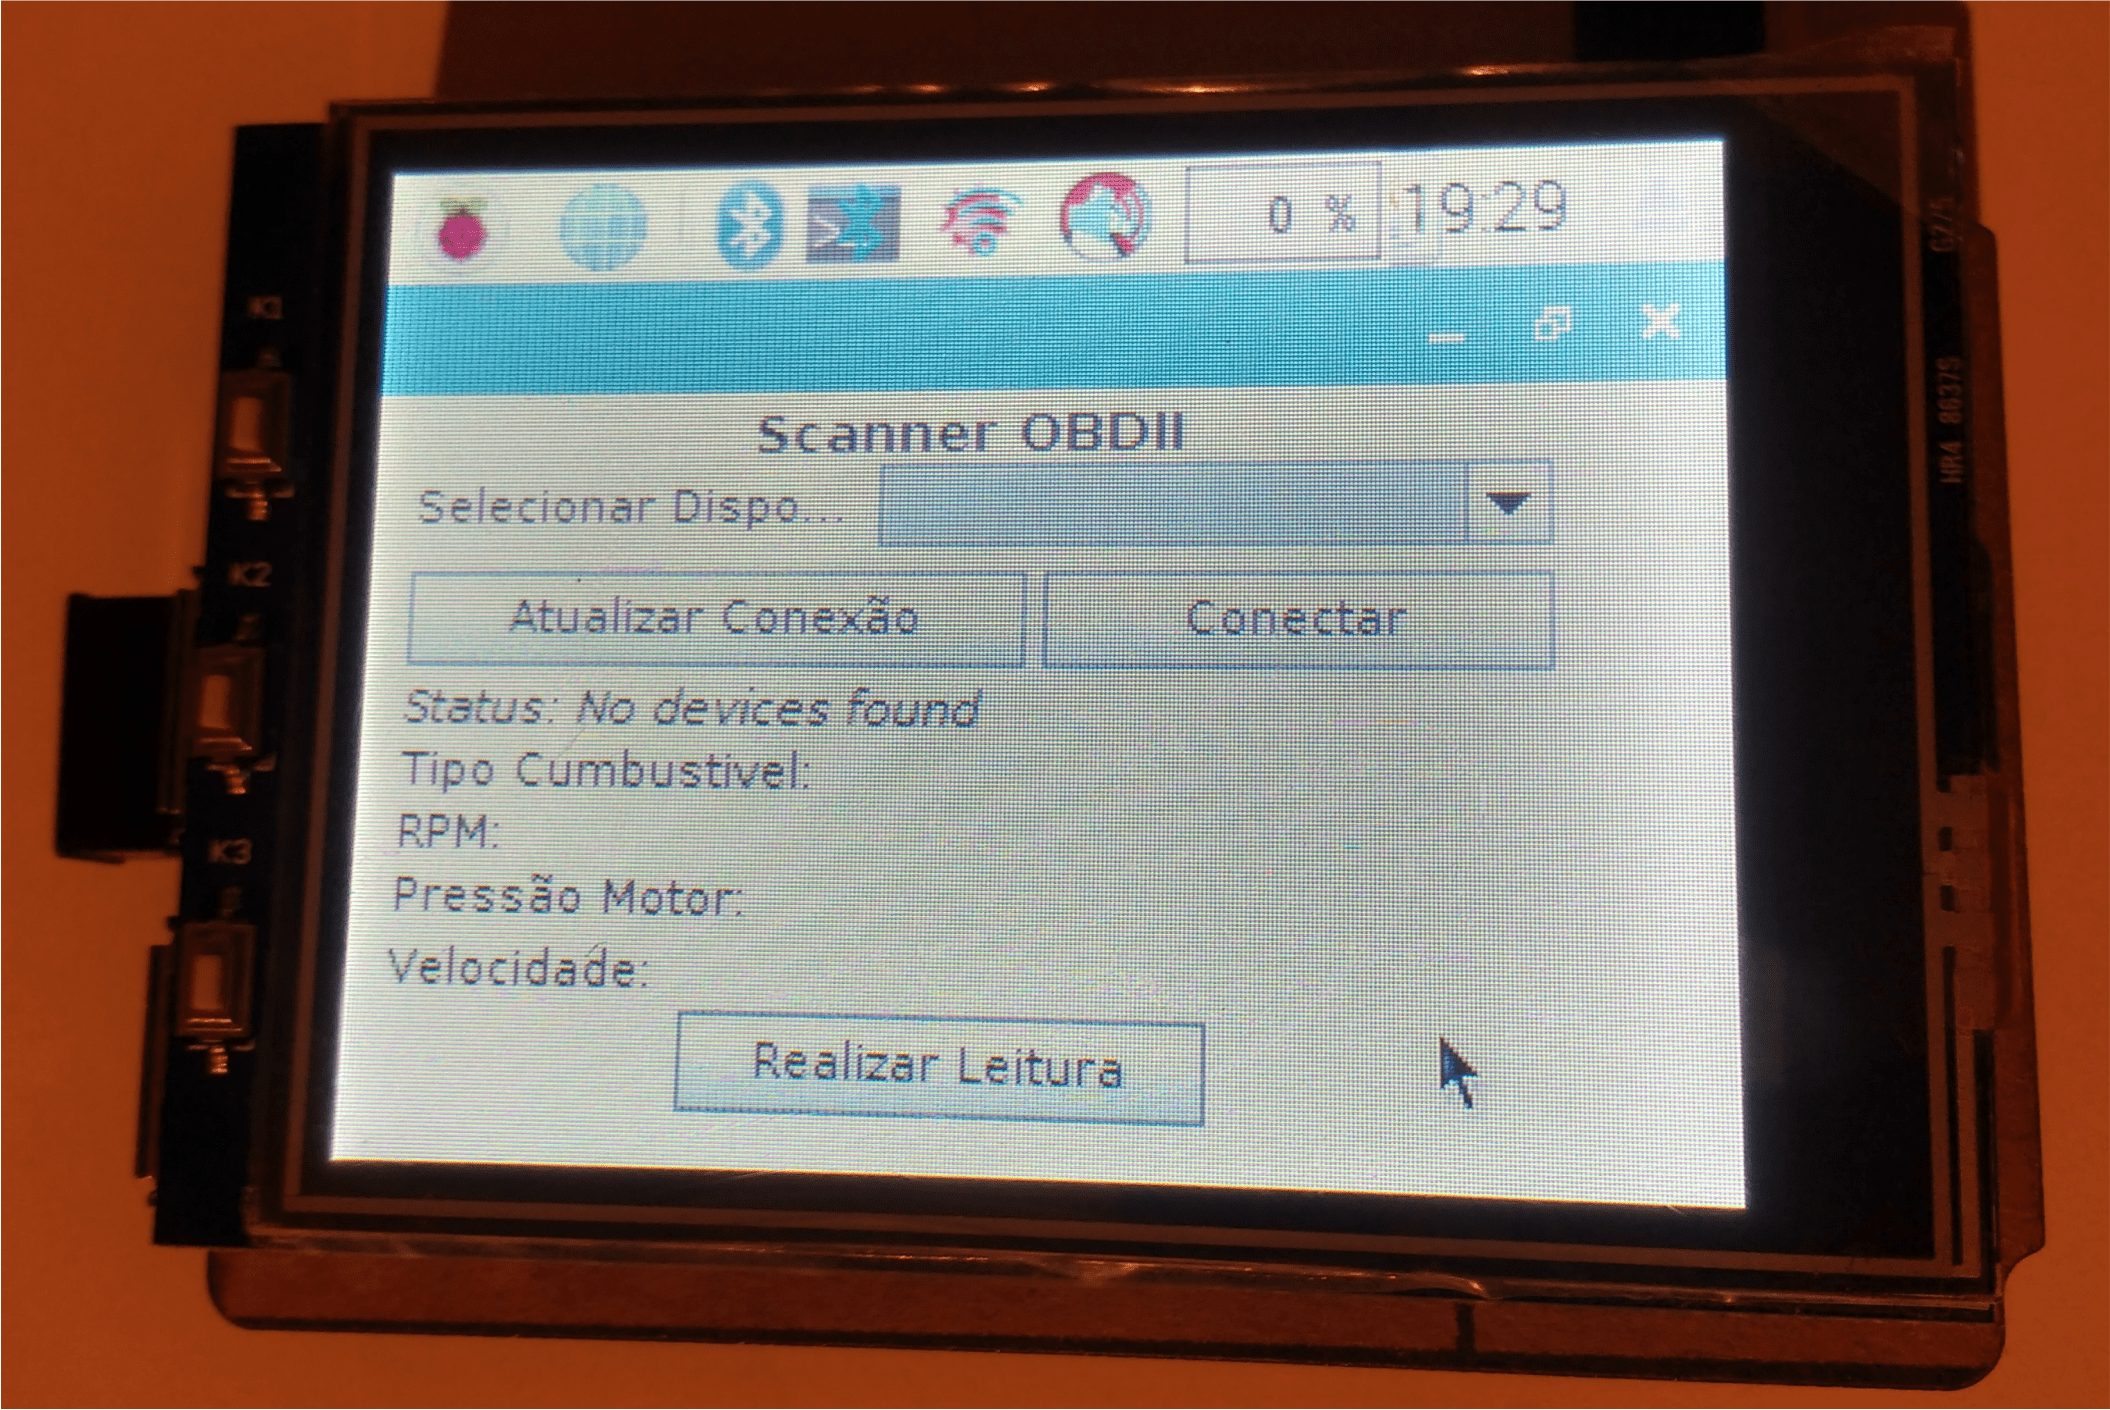
\includegraphics[scale=.15]{imagens/sistemaRodandoRaspberry-min.png}}\\
\makebox[\width]{Fonte: produzido pelo autor} \label{Fig:raspberry_sistema}
\end{figure}

\section{INTEGRAÇÃO DA APLICAÇÃO COM SERVIÇO DE COMPUTAÇÃO EM NUVEM}
Primeiramente foi feita uma análise da arquitetura que o servidor deveria possuir além de levantar quais serviços e software seriam necessários para garantir o funcionamento do sistema na web. Baseando-se nestas informações, foi adquirido um servidor do tipo \textit{Elastic Compute Cloud (EC2)} da Amazon, pertencente à categoria t2.micro, contendo 1Gb de memória RAM, processador Intel Xeon de 2.5GHz e 8Gb de armazenamento do tipo \textit{Elastic Block Store (EBS)}, rodando o sistema operacional Ubuntu \textit{Server} 16.04 LTS. Esta categoria de servidor permite o uso por um ano de forma gratuita. O \textit{EC2}, segundo a \citeonline{amazonec2}, é um \textit{web service} que disponibiliza capacidade computacional segura e redimensionável na nuvem. O \textit{EBS} disponibiliza volumes de armazenamento para uso com instâncias de servidores do tipo \textit{EC2} \nocite{amazonebs}.

\subsection{INSTALAÇÃO E CONFIGURAÇÃO DA BASE DE DADOS NA NUVEM}
Depois de feita a aquisição do servidor, a próxima etapa foi instalar e configurar um serviço de banco de dados. Para esta situação foi escolhido o MongoDB, que é um banco de dados não relacional baseado em documentos \textit{JSON} \cite{mongodbwhatis}. Este banco possui um esquema de dados flexível, permitindo o mapeamento de um documento para uma entidade ou objeto. Cada documento é armazenado dentro de uma coleção do banco. De acordo com o manual do \citeonline{mongodbdatamodeling}, os modelos de dados desnormalizados permitem que as aplicações alterem a estrutura dos documentos contidos nas coleções durante o armazenamento de dados realizando apenas uma única operação no banco de dados sem se preocupar com a sua remodelagem.

Logo após a instalação do banco, foi criado uma base de dados no MongoDB com o nome \textit{car\_monitor}, e dentro desta base, foi criado uma coleção com o nome \textit{reading\_sensors}. Esta coleção armazenará todos os dados do veículo que foram lidos pelo \textit{Raspberry Pi}. A Figura \ref{Fig:base_dados} representa a estrutura do banco de dados que será responsável por armazenar as informações.

\begin{figure}[!ht]
\centering
\caption{Foto da estrutura do banco de dados.} 
{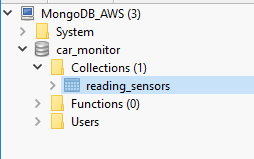
\includegraphics[scale=1.5]{imagens/baseDadosBanco.png}}\\
\makebox[\width]{Fonte: produzido pelo autor} \label{Fig:base_dados}
\end{figure}

\subsection{INTEGRAÇÃO DO SOFTWARE COM A BASE DE DADOS}
Para a integração do software com a base de dados foi necessário instalar as seguintes dependências do MongoDB no projeto: \textit{mongodb-driver}, \textit{mongodb-driver-core} e \textit{bson}, todas na versão 3.5. Para manipular as informações no banco de dados pelo software, foi decidido seguir o modelo \textit{Data Access Object (DAO)}. Segundo a definição de \apudonline{deepak}{medeirosdao}, o padrão \textit{DAO} abstrai e encapsula todos os acessos ao banco de dados, gerenciando a conexão com a base para obter e armazenar as informações. Para implementar este padrão, foi necessário alterar a estrutura do projeto, com a criação de 3 pacotes adicionais: o pacote \textit{dao}, o pacote \textit{database} e o pacote \textit{models}. A Figura \ref{Fig:diagrama_classe_novo} mostra a nova estrutura de pacotes e a Figura \ref{Fig:diagrama_mvc_dao} exibe a representação dos padrões utilizados no projeto baseado nos pacotes implementados.

\begin{figure}[!ht]
\centering
\caption{Diagrama de pacote exibindo a nova estrutura de pacotes do projeto com as respectivas classes.} 
{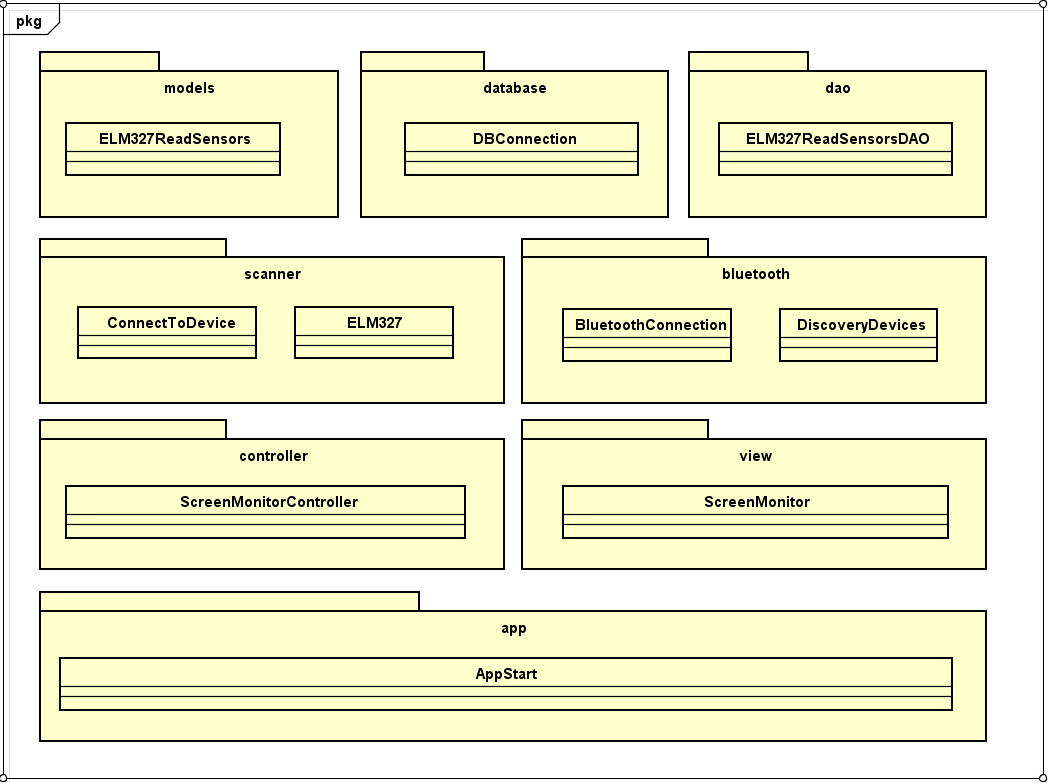
\includegraphics[scale=.44]{imagens/estruturacaoPacotesNovo.png}}\\
\makebox[\width]{Fonte: produzido pelo autor} \label{Fig:diagrama_classe_novo}
\end{figure}

\begin{figure}[!ht]
\centering
\caption{Representação da arquitetura \textit{MVC} com o padrão \textit{DAO} do projeto.} 
{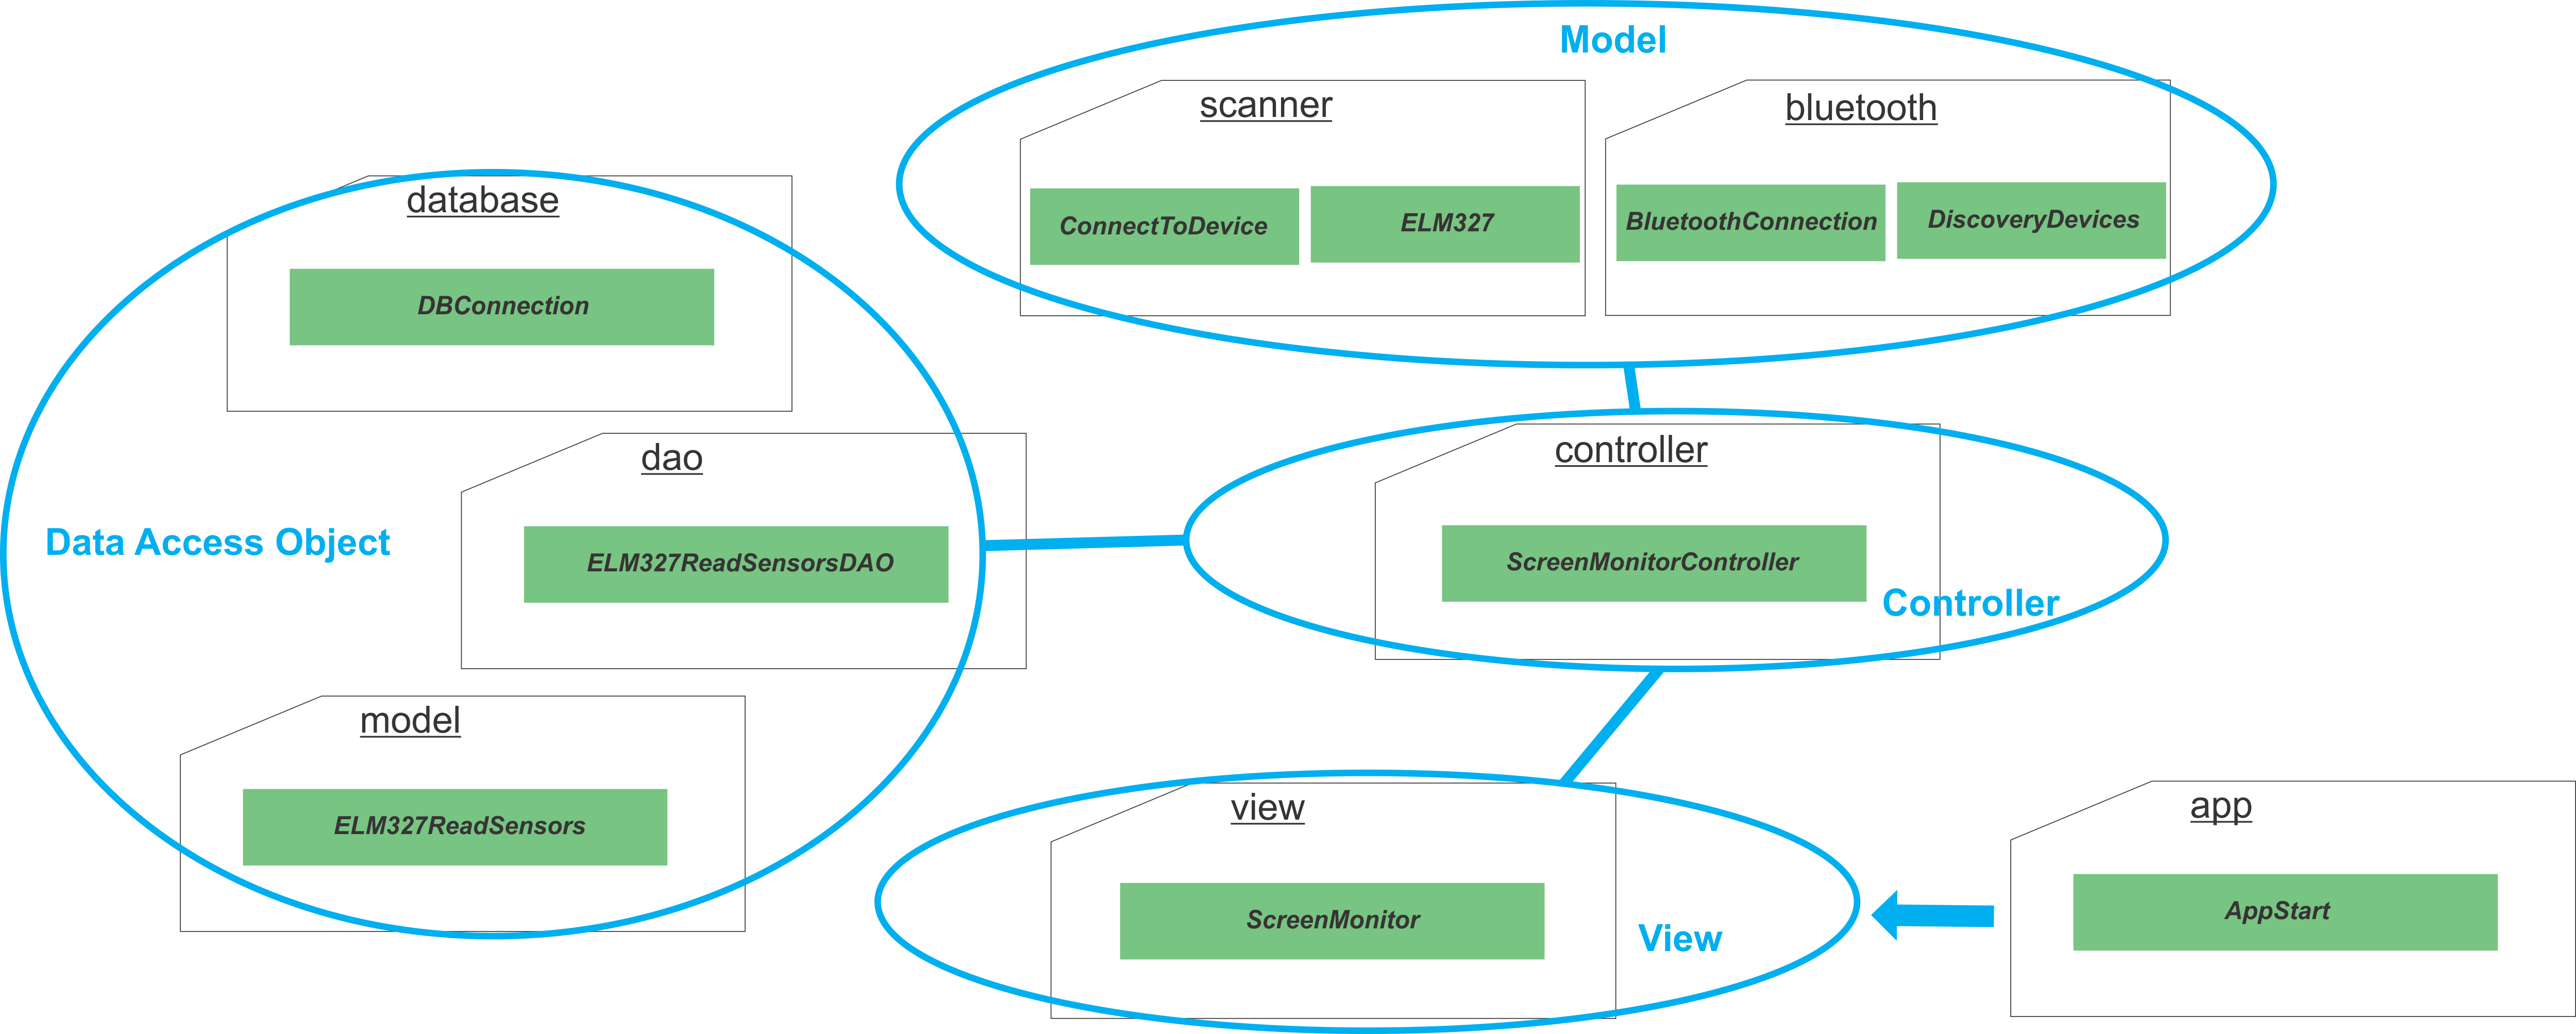
\includegraphics[scale=.38]{imagens/diagramaMvcDao.png}}\\
\makebox[\width]{Fonte: produzido pelo autor} \label{Fig:diagrama_mvc_dao}
\end{figure}

O pacote \textit{model} contém a classe modelo \textit{ELM327ReadSensors} (Figura \ref{Fig:elm327_read_sensors}), que será utilizada para a criação de objetos que armazenarão todas as informações que foram lidas do veículo. Esta classe possui os campos do tipo \textit{string} referentes à estas informações, que são: modeloCarro, chassiCarro, rpm, velocidade, pressaoCombustivel e tipoCombustivel.

\begin{figure}[!ht]
\centering
\caption{Foto da classe \textit{ELM327ReadSensors}.} 
{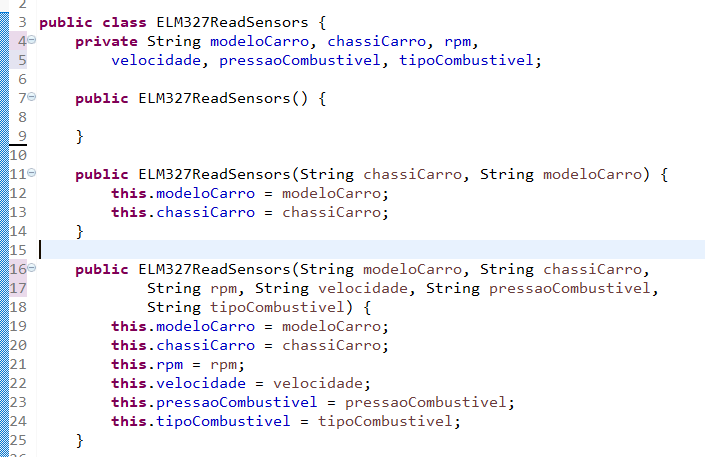
\includegraphics[scale=.66]{imagens/pacoteModel-ELM327ReadSensors.png}}\\
\makebox[\width]{Fonte: produzido pelo autor} \label{Fig:elm327_read_sensors}
\end{figure}

Analisando o pacote \textit{database}, ele traz a classe \textit{DBConnection} (Figura \ref{Fig:db_connection}) que é responsável por criar a conexão com o banco de dados na nuvem. Esta classe contém o método estático \textit{getConnection} que retorna um objeto do tipo \textit{MongoDatabase}, pertencente à biblioteca \textit{mongodb-driver}.

\begin{figure}[!ht]
\centering
\caption{Foto da classe \textit{DBConnection}.} 
{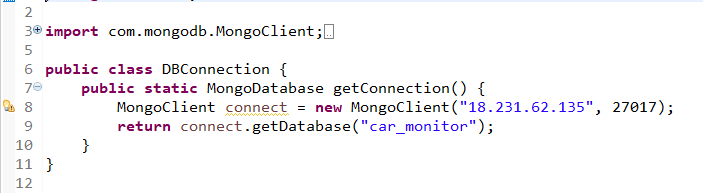
\includegraphics[scale=.66]{imagens/pacoteDatabase-DBConnection.png}}\\
\makebox[\width]{Fonte: produzido pelo autor} \label{Fig:db_connection}
\end{figure}

No pacote \textit{dao}, existe a classe \textit{ELM327ReadSensorsDAO} (Figura \ref{Fig:elm327_read_sensors_dao}), que implementa o padrão \textit{DAO}. Esta classe abstrai o acesso ao banco de dados, fornecendo um método para inserção chamada \textit{insertDB}, que recebe como parâmetro um objeto do tipo \textit{ELM327ReadSensors}. Este método é responsável por receber este objeto e estruturá-lo em um outro objeto no formato \textit{BSON} para ser inserido no banco de dados. Os dados contidos no MongoDB são documentos \textit{JSON} codificados, conhecidos como \textit{BSON} \cite{mongodbjsonbson}.

\begin{figure}[!ht]
\centering
\caption{Foto da classe \textit{ELM327ReadSensorsDAO}.} 
{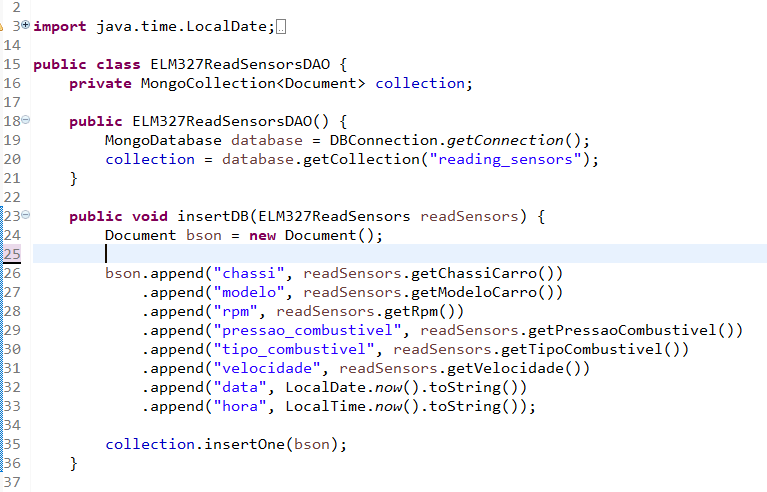
\includegraphics[scale=.66]{imagens/pacoteDao-ELM327ReadSensorsDAO.png}}\\
\makebox[\width]{Fonte: produzido pelo autor} \label{Fig:elm327_read_sensors_dao}
\end{figure}

Para permitir o upload dos dados na nuvem utilizando o \textit{Raspberry Pi}, foi levantado a necessidade de utilizar uma rede móvel 4G. Desta forma, seria possível conectar o software com o MongoDB localizado em uma instância da Amazon na nuvem.

\subsection{INSTALAÇÃO E CRIAÇÃO DO \textit{WEB SERVICE}}
Depois de integrado o software com o banco de dados, foi necessário criar um \textit{web service} que seria responsável por realizar as consultas no banco e disponibilizá-las para alguma outra aplicação poder consumir estas informações. Baseado nesta definição, foi escolhido a plataforma Node.js na versão 6.11 para a criação do \textit{web service} utilizando a linguagem \textit{JavaScript}. Segundo o \citeonline{w3schools}, o Node.js é uma plataforma para servidor de código aberto que utiliza a linguagem \textit{JavaScript} para as aplicações de \textit{web service}, permitindo a manipulação de informações no \textit{backend}.

Foi necessário a instalação de três pacotes do Node.js para a criação do \textit{web service}: o pacote \textit{express}, responsável pela abstração das rotas, o pacote \textit{body-parser} responsável por efetuar as conversões \textit{JSON} e o pacote \textit{mongoose}, responsável por mapear os objetos do MongoDB. O \textit{web service} foi implementado apenas para requisições HTTP do tipo \textit{GET} na rota \textit{‘/collection’}. Desta maneira, qualquer aplicação que fazer uma solicitação do tipo \textit{GET} para esta rota, será chamado uma função no \textit{web service} (Figura \ref{Fig:get_collection}) que é responsável por realizar a consulta no banco de dados e retornar os valores encontrados em formato de uma lista de objetos \textit{JSON} respondendo à requisição.

\begin{figure}[!ht]
\centering
\caption{Foto do método js responsável por responder a solicitações \textit{GET} na rota \textit{'/collection'}.} 
{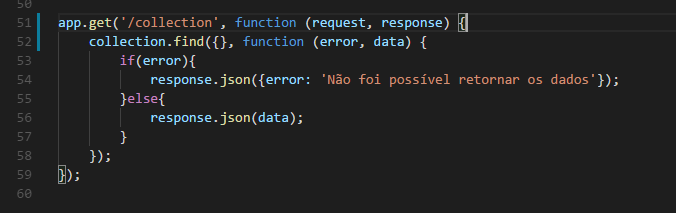
\includegraphics[scale=.66]{imagens/GET-collection_webservice.png}}\\
\makebox[\width]{Fonte: produzido pelo autor} \label{Fig:get_collection}
\end{figure}

\subsection{INSTALAÇÃO E CONFIGURAÇÃO DO SERVIDOR WEB E CRIAÇÃO DA PÁGINA}
Após concluída a etapa anterior, seria preciso instalar um servidor web para hospedar a página que iria consumir os dados disponibilizados pelo \textit{web service}. Foi escolhido o servidor Apache para esta finalidade. As configurações padrão do servidor Apache foram mantidas, pois não haveria necessidade de alterá-las nesta situação.

O desenvolvimento da página web foi feito utilizando-se as tecnologias HTML, \textit{JQuery} e \textit{Bootstrap}. A função desta página é simplesmente consumir as informações disponíveis no \textit{web service}, não possuindo nenhuma outra funcionalidade específica. A página contém um componente de seleção, que permite escolher o tipo de filtro para exibir os resultados. Logo abaixo contém o campo de entrada que permite inserir o valor da informação que se deseja filtrar. A Figura \ref{Fig:input_fitros} apresenta os componentes de filtro mencionados acima.

\begin{figure}[!ht]
\centering
\caption{Foto dos elementos de filtro da página.} 
{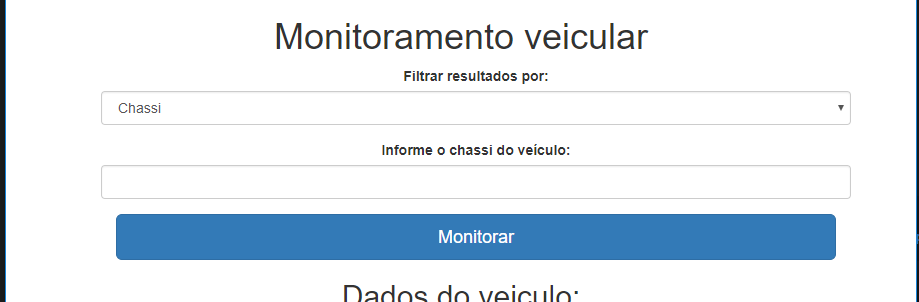
\includegraphics[scale=.62]{imagens/paginaweb_inputs.png}}\\
\makebox[\width]{Fonte: produzido pelo autor} \label{Fig:input_fitros}
\end{figure}

Após preenchido o valor, existe um botão chamado monitorar, que ao acionado, faz a requisição \textit{GET} via \textit{AJAX} (Figura \ref{Fig:requisicao_ajax}) para o \textit{web service} e retorna os valores na tabela de acordo com o filtro informado.
Por fim, a Figura \ref{Fig:arquitetura_projeto} mostra toda a integração do sistema com a nuvem, representando as trocas de dados e comunicação entre diferentes serviços.

\begin{figure}[!ht]
\centering
\caption{Foto do método \textit{JQuery} responsável pelo \textit{AJAX}.} 
{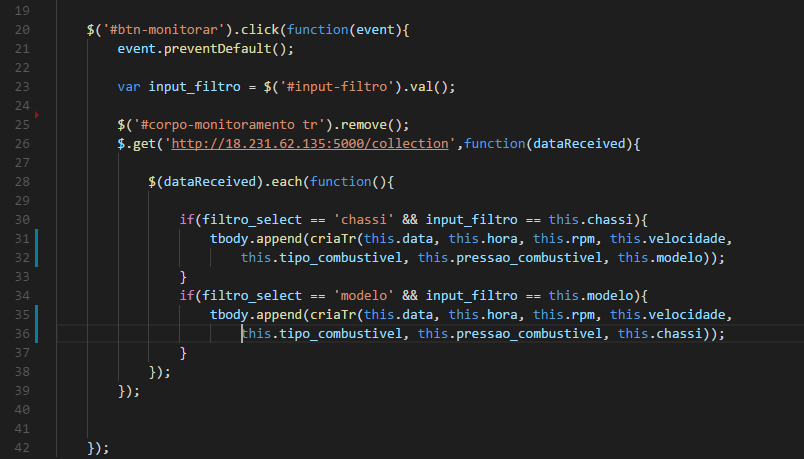
\includegraphics[scale=.64]{imagens/requisicaoAjax.png}}\\
\makebox[\width]{Fonte: produzido pelo autor} \label{Fig:requisicao_ajax}
\end{figure}

\begin{figure}[!ht]
\centering
\caption{Diagrama representando a comunicação do sistema com a nuvem.} 
{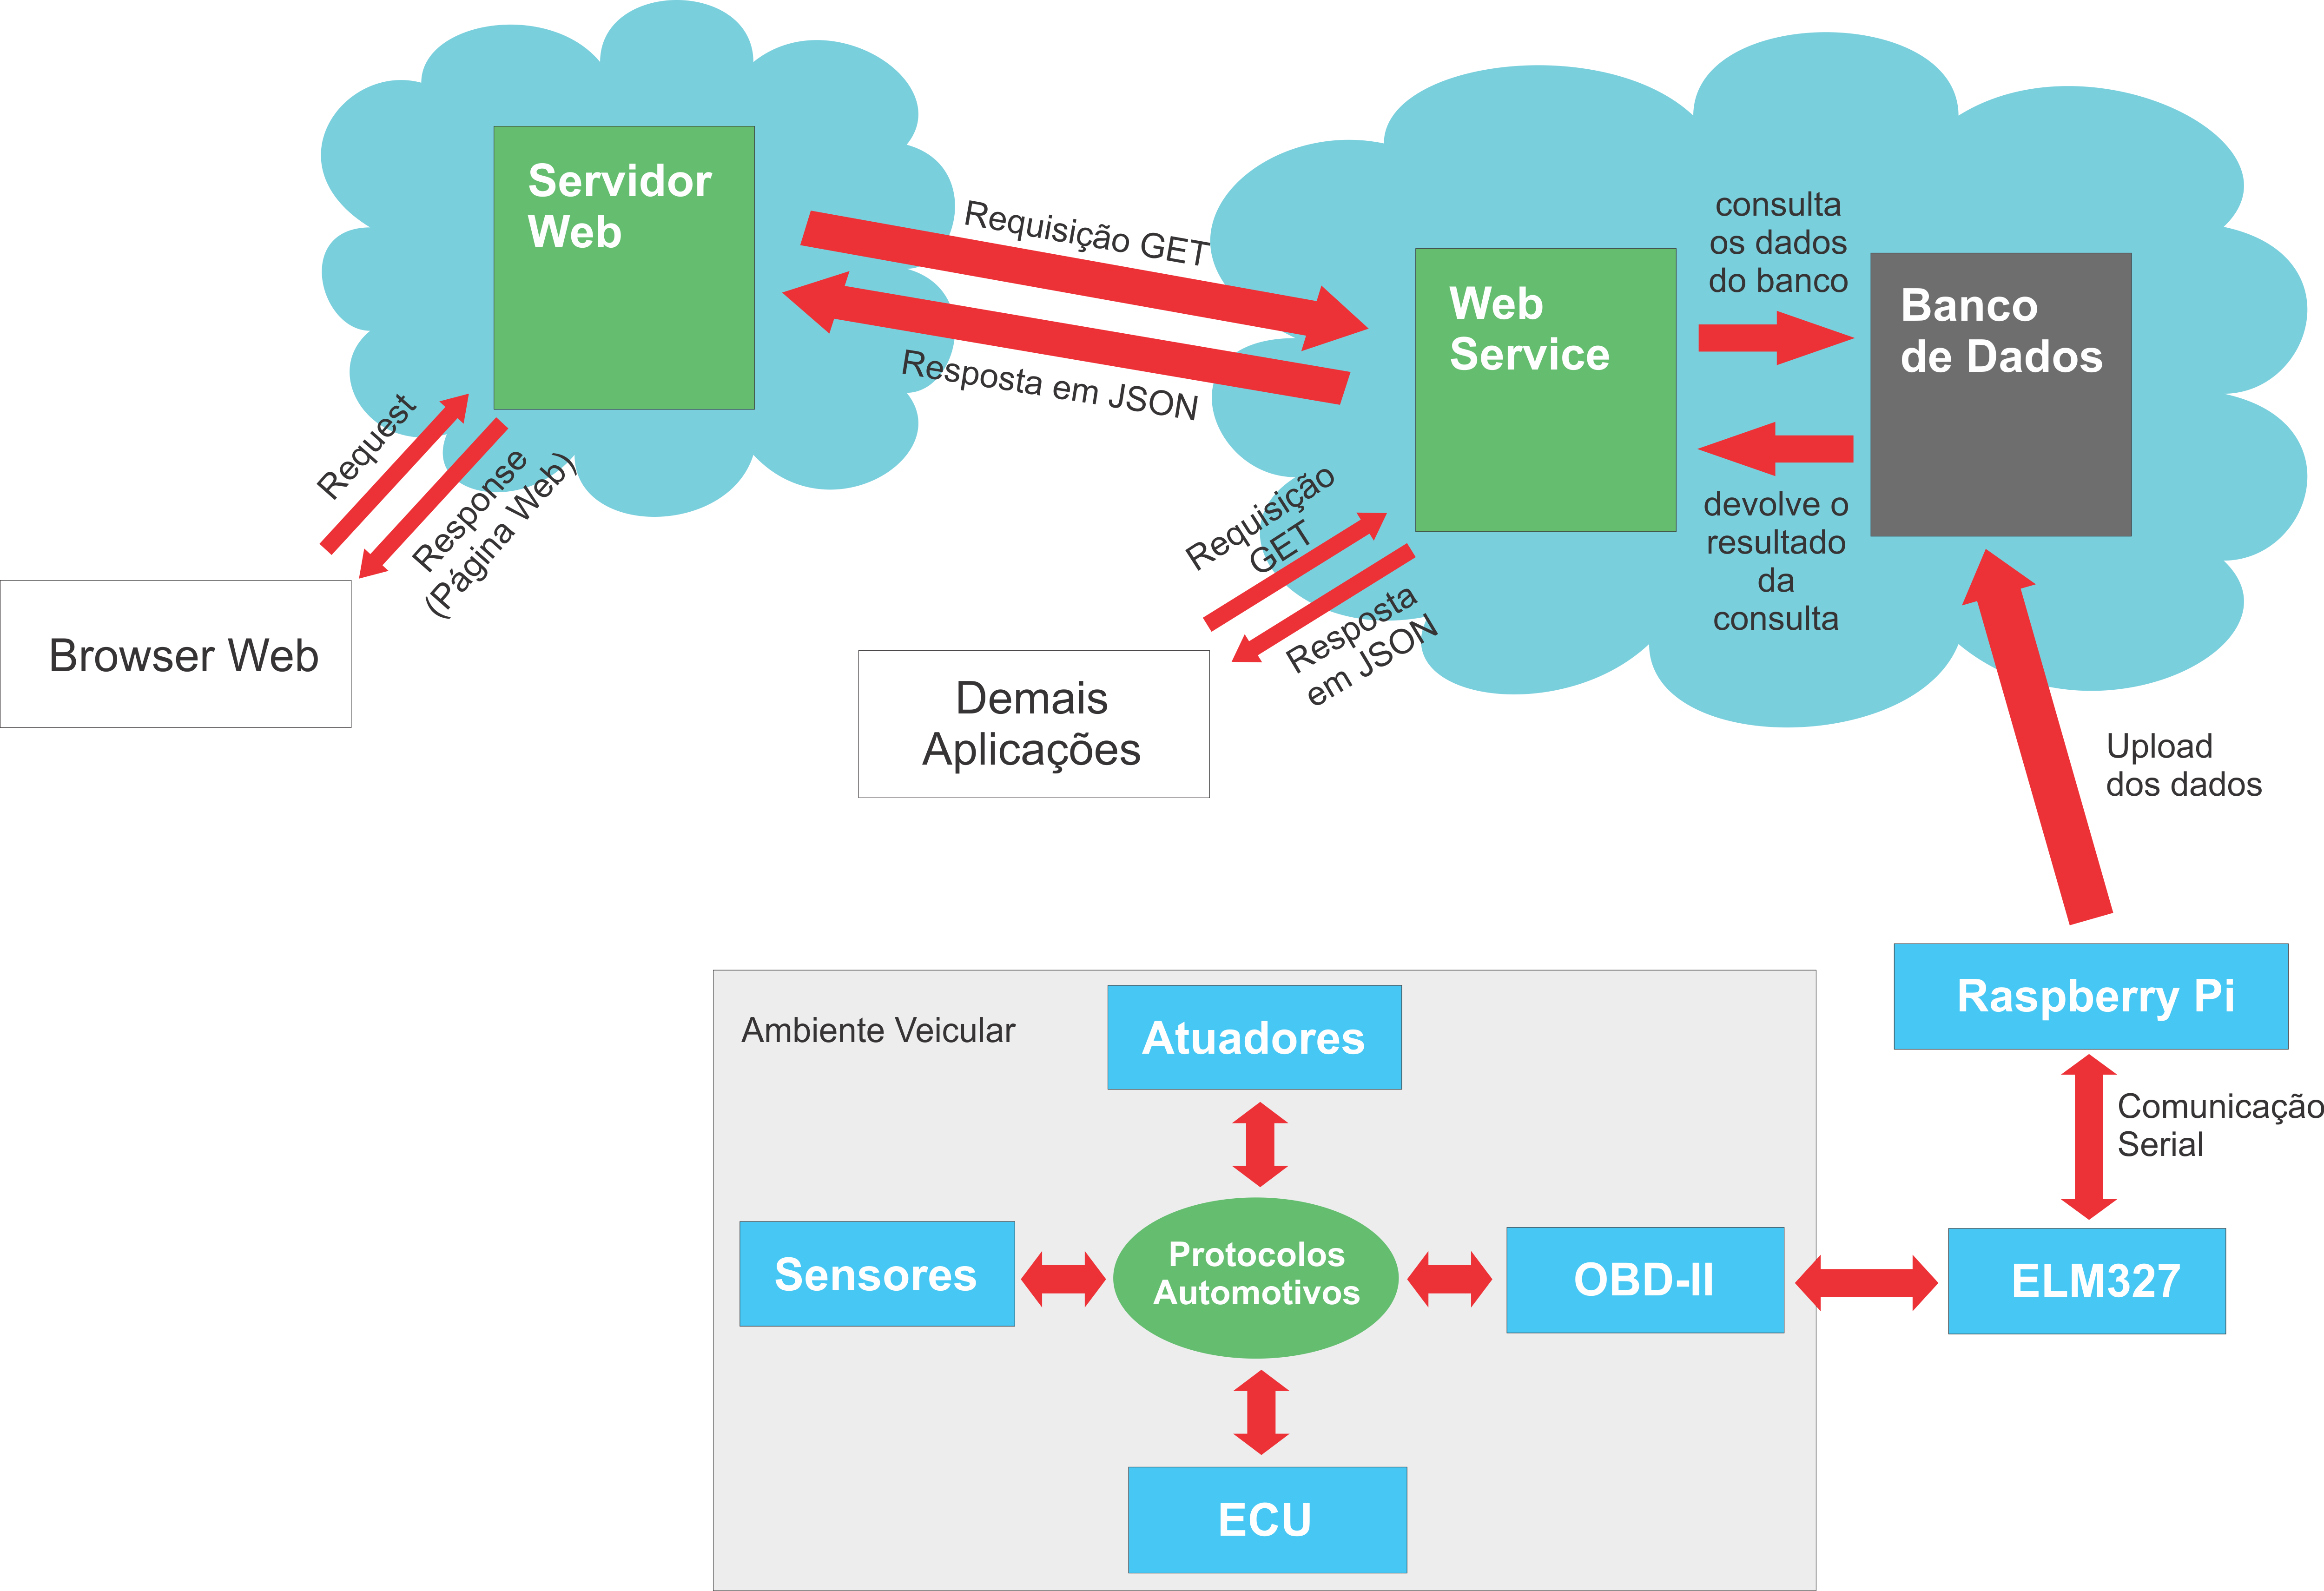
\includegraphics[scale=.38]{imagens/arquiteturaRedeVeicularELM327Nuvem.png}}\\
\makebox[\width]{Fonte: produzido pelo autor} \label{Fig:arquitetura_projeto}
\end{figure}
